\documentclass[a4paper,11pt,fleqn]{article}%fleqn pour aligner les equations à gauche
\usepackage{/home/rweye/Nextcloud/Documents/Overleaf/Styles/Cours}


\newcommand{\chnum}{Chapitre 2}
\newcommand{\chtitle}{Composition des solutions aqueuses}
\newcommand{\dtype}{Cours}

\begin{document}
\maketitle

\section{La concentration}
	\subsection{Définitions}
	Une solution est un mélange à l'état liquide. il est constitué d'un solvant, qui est l'espèce chimique majoritaire, et d'un soluté qui est une espèce dispersée dans le solvant.\\
	$$\text{Solution} = \text{Solvant} + \text{soluté}$$
	\textcolor{green!50!black}{Exemple : eau salée = eau + chlorure de sodium (\ce{NaCl})\\
	solution de glucose = eau + glucose (\ce{C6H12O6})}
	
	\subsection{Concentration en soluté}
	La concentration en masse d'un soluté est la masse de soluté dissous dans un volume de solution. $$\gamma = \dfrac{m_{\text{soluté}}}{V_{\text{solution}}}$$
	avec $m$ en grammes, $V$ en litres et $\gamma$ en \unit{\gram\per\liter}.\\
	\textcolor{green!50!black}{Exemple : On dissout 2 carrés de sucre de \SI{8}{g} dans 1/2 L d'eau. Quelle sera la concentration de la solution de saccharose ainsi créée ?}\\
	
	\vspace*{2cm}
	
	Il faut faire attention à bien distinguer la concentration et la masse volumique : les unités sont identiques mais la concentration utilise la masse de soluté alors que la masse volumique utilise la masse totale de la solution.\\
	\textcolor{green!50!black}{Exemple : $\gamma_{sucre}(sirop)$ = \SI{20}{\gram\per\liter}  alors que $\rho(sucre)$ = \SI{1180}{\gram\per\liter}.}
	
	\subsection{Solubilité}
	On ne peut pas dissoudre une quantité illimitée de soluté dans un volume de solvant. Lorsqu'on atteint cette limite on dit que la solution est \textbf{saturée}.\\
	La solubilité est la concentration à partir de laquelle on ne peut plus dissoudre d'avantage de soluté. C'est donc la concentration maximale d'un soluté dans un volume de solvant donné.\\
	\textcolor{green!50!black}{Exemple : Saccharose : $\gamma_{max}$ = \SI{2000}{\gram\per\liter}\\
	Chlorure de sodium : $\gamma_{max}$ = \SI{358,5}{\gram\per\liter}\\
	Sulfate d'argent : $\gamma_{max}$ = \SI{520E-6}{\gram\per\liter}}\\
	Remarque :
	\begin{itemize}
		\item la solubilité varie avec la température (plus la température augmente, plus une espèce peut se solubiliser)
		\item une solution peut être saturée pour un soluté et pas pour un autre.
	\end{itemize}
	\textcolor{purple!50!black}{Exercice : Quelle est la masse maximale de chlorure de sodium pouvant se dissoudre dans une piscine de \SI{8}{m} de long, \SI{4}{m} de large et \SI{1,5}{m} de profondeur ?}
	\vspace{2cm}

\section{Préparer une solution}
	\subsection{Par dissolution}
	La dissolution est la fait de disperser un soluté dans un solvant. Le soluté peut être à l'état solide (exemple du sucre) ou gazeux (exemple du \ce{CO2} des boissons gazeuses).\\
	On procède  en mesurant une masse de soluté  que l'on additionne au solvant en agitant de manière à favoriser la dispersion. Il est possible de chauffer pour accélérer la dissolution.
	\subsection{Par dilution}
	La dilution permet de préparer une solution de concentration donnée à partir d'une solution plus concentrée (appelée solution mère). Il s'agit de mesurer un volume précis de solution mère dans lequel on ajoutera du solvant pur.\\
	\textcolor{green!50!black}{Exemple : l'ajout d'eau dans un café trop fort.}
	\subsection{Conservation de la masse}
	Quelle que soit la technique utilisée, la masse de soluté utilisée se retrouve dans la solution finale. Lors d'une dissolution la masse mesurée de soluté se retrouve dans la solution : $$m_{\text{soluté pesé}} = m_{\text{soluté en solution}} = \gamma \times V_{solution}$$
	Lors d'une dilution, la masse de soluté de la solution mère prélevée se retrouve dans la solution fille : $$m_{\text{mère}} = m_{\text{fille}}$$ donc $$\gamma_{\text{mère}} \times V_{\text{mère}} = \gamma_{\text{fille}}\times V_{\text{fille}}$$

\section{Déterminer la concentration d'une solution}
	\subsection{Échelle de teinte}
	Lorsqu'une solution colorée est diluée, sa teinte devient de plus en plus claire. En préparant plusieurs solutions à des concentrations différentes, on peut déterminer la concentration d'une solution (pour un même soluté) en comparant sa teinte à celle des solutions de référence. On peut ainsi obtenir un encadrement de la concentration de la solution.
\begin{figure}[h!]
	\begin{center}
	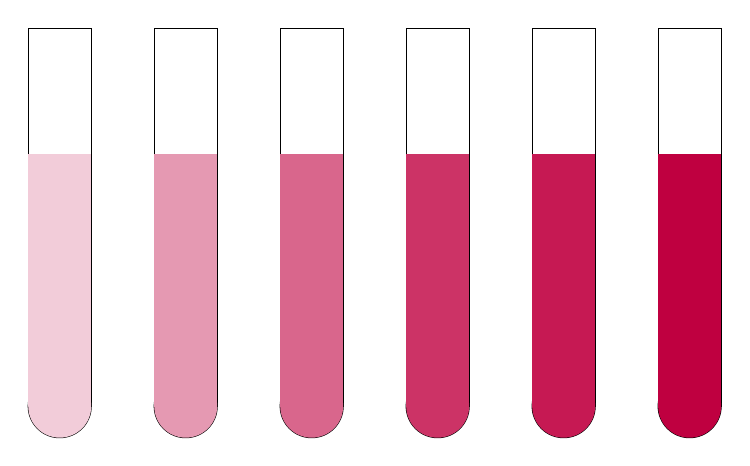
\begin{tikzpicture}[scale=.8, transform shape]
	\draw (0,0) rectangle (0+1,6); \draw(0+0.5,0) circle (.5);\fill[purple!20] (0,0) rectangle (0+1,4);\fill[purple!20] (0+0.5,0) circle (.5);
	\draw (2,0) rectangle (2+1,6); \draw(2+0.5,0) circle (.5);\fill[purple!40] (2,0) rectangle (2+1,4);\fill[purple!40] (2+0.5,0) circle (.5);
	\draw (4,0) rectangle (4+1,6); \draw(4+0.5,0) circle (.5);\fill[purple!60] (4,0) rectangle (4+1,4);\fill[purple!60] (4+0.5,0) circle (.5);
	\draw (6,0) rectangle (6+1,6); \draw(6+0.5,0) circle (.5);\fill[purple!80] (6,0) rectangle (6+1,4);\fill[purple!80] (6+0.5,0) circle (.5);
	\draw (8,0) rectangle (8+1,6); \draw(8+0.5,0) circle (.5);\fill[purple!90] (8,0) rectangle (8+1,4);\fill[purple!90] (8+0.5,0) circle (.5);
	\draw (10,0) rectangle (10+1,6); \draw(10+0.5,0) circle (.5);\fill[purple] (10,0) rectangle (10+1,4);\fill[purple] (10+0.5,0) circle (.5);
	%draw[->,>=latex] (L) to[bend left] (S);
	%\draw[->,>=latex] (S) to[bend left] (P);
	\end{tikzpicture}
	\caption{Échelle de teinte pour le permanganate de potassium (\ce{KMnO4})}
	\end{center}
	\end{figure}
	
\newpage
	\subsection{Courbe d'étalonnage}
	Il est possible de déterminer la concentration d'une solution à partir d'une grandeur physique (exemple la masse volumique) en réalisant une courbe d'étalonnage.\\
	Lorsque l'on représente graphiquement une grandeur physique en lien avec la concentration et la concentration d'une solution, on peut observer une droite.\\
	La courbe d'étalonnage est obtenue en réalisant une série de solutions d'un soluté donné avec des concentrations différentes. On mesure la grandeur physique sélectionnée, puis on trace la courbe $G = f(\gamma)$. Pour être plus précis, il faut réaliser de nombreuses mesures pour tracer la courbe d'étalonnage. On peut alors modéliser la courbe, c'est à dire déterminer l'équation correspondant à la droite tracée.
	
	\begin{figure}[h!]
	\begin{center}
	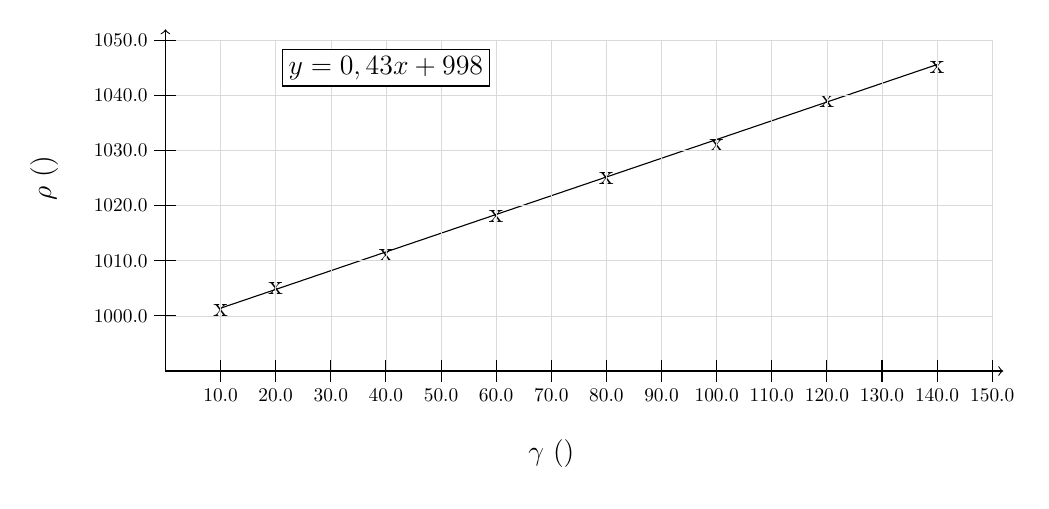
\begin{tikzpicture}[scale = .7,transform shape]
	\draw (1.0,100.1) node{\Large x};
	\draw (2.0,100.5) node{\Large x};
	\draw (4.0,101.1) node{\Large x};
	\draw (6.0,101.8) node{\Large x};
	\draw (8.0,102.5) node{\Large x};
	\draw (10.0,103.1) node{\Large x};
	\draw (12.0,103.9) node{\Large x};
	\draw (14.0,104.5) node{\Large x};
	\draw [domain=1:14] plot(\x,{0.34*\x + 99.8});
	\draw [very thin, gray!30](0,99) grid[step = 1] (15,105);
	\draw [->] (0,99) -- (0,105.2);
	\draw [->] (0,99) -- (15.2,99);
	\foreach \k in {1,...,15}
		{\draw (\k,98.8)--(\k,99.2);
		\pgfmathsetmacro{\labs}{\k*10}
		\draw (\k,98.8) node[below] {\labs};
		}
	\foreach \k in {100,...,105}
		{\draw (-.2,\k)--(.2,\k);
		\pgfmathsetmacro{\labs}{\k*10}
		\draw (-.2,\k) node[left] {\labs};}
	\clip (-2.5,97) rectangle (15,105);
	\node[draw,rectangle,fill=white] (A) at (4,104.5) {\Large $y = 0,43 x + 998$};
	\node[rotate =90] (Y) at (-2.2,102.5) {\Large $\rho$ (\unit{\gram\per\liter})};
	\node (X) at (7,97.5) {\Large $\gamma$ (\unit{\gram\per\liter})};
	\end{tikzpicture}
	\caption{Exemples de droites d'étalonnage pour la masse volumique en fonction de la concentration en saccharose d'une solution}
	\end{center}
	\end{figure}
	
\end{document}
